

\begin{exercise}\label{exer:51}
A ``focus-inversive'' polygon, is a $N$-gon whose vertices are inversions of elliptic billiard N-periodic vertices with respect to a circle of radius $\rho$ centered on one focus. See \cref{fig:chap5_inversiveN3}.

\begin{figure}[H]
    \centering
    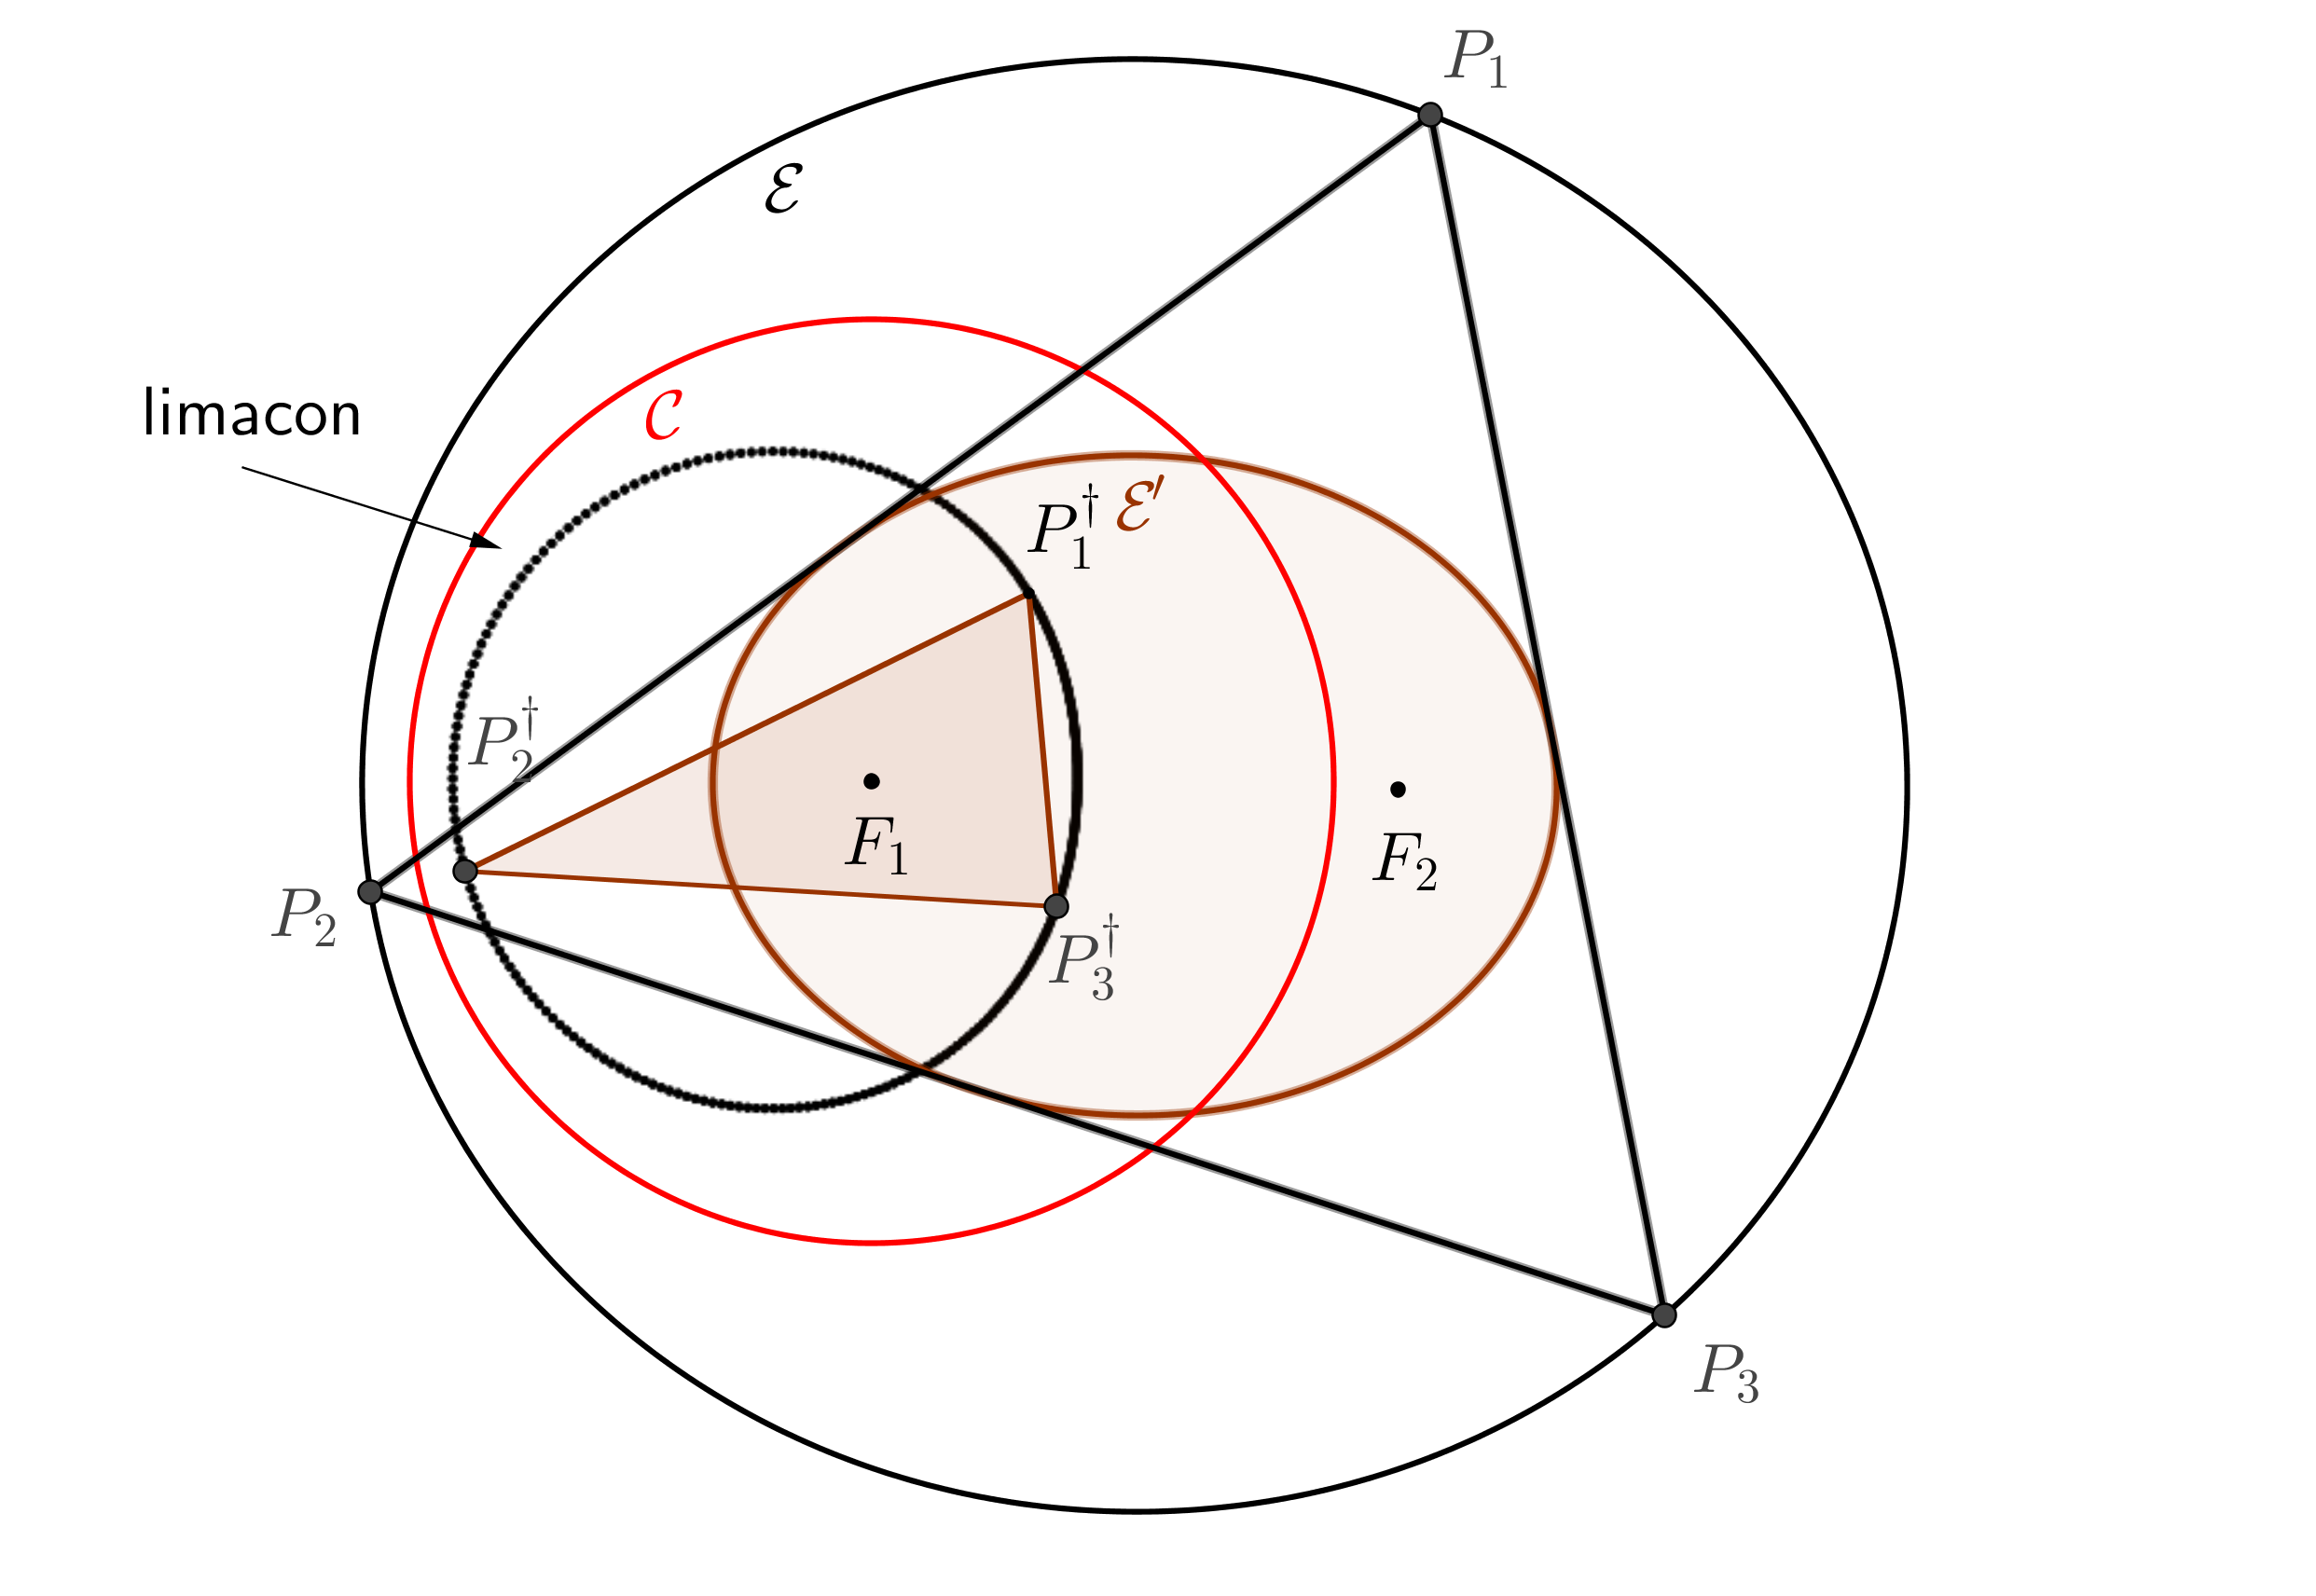
\includegraphics[scale=0.5]{pics_05_0910_inversivoN3.png}
    \caption{Inversive triangle $P_1^{\dag}P_2^{\dag}P_3^{\dag}$ of 3-billiard orbit $P_1P_2P_3$.}
    \label{fig:chap5_inversiveN3}
\end{figure}

It is well known the inversion of an ellipse with respect to a focus-centered unit circle is Pascal's Limaçon $\mathcal{L}(t)$ \cite{ferreol2020-limacon}, given by:

\[ \mathcal{L}(t)=\left[-a \cos{t} (\varepsilon  \cos{t}+1)-c,a \sin{t} (\varepsilon \cos{t}+1)\right],\;\;0{\leq}t{\leq}2\pi
\]

\noindent Therefore:

For any $N$, the focus-inversive family is inscribed in $\mathcal{L}(t)$.

\noindent i) Show that 
the perimeter $L^\dagger$ of the N=3 focus-inversive family is invariant and given by:

\[L^\dagger=\rho^2 \frac {\sqrt { \left( 8\,{a}^{4}+4\,{a}^{2}{b}^{2}+2\,{b}^{4}
 \right) \delta+8\,{a}^{6}+3\,{a}^{2}{b}^{4}+2\,{b}^{6}}}{{a}^{2}{b}^{
2}}\]
 
\noindent ii) Show that for $N=3$, the sum of focus-inverse spoke lengths $\sum{1/d_{1,i}}$ is invariant and given by:

\[  \sum{1/d_{1,i}}=\frac {{a}^{2}+{b}^{2}+\delta}{a{b}^{
2}}
\] 

\noindent iii) Show that for $N=3$, the sum of focus-inversive cosines $\sum\cos{\theta_{1,i}^\dagger}$ is given by:
\[\sum\cos{\theta_{1,i}^\dagger}=\frac{\delta (a^2+c^2-\delta)}{a^2c^2}\]

%\noindent iv) Show that the product of the areas for $N=3$ of the inversive triangle is invariant under the family of 3-periodic orbits.

\end{exercise}


\begin{exercise}\label{exer:52} Let $X_1^{\dag}$ be the incenter of the inversive triangle $P_1^{\dag}P_2^{\dag}P_3^{\dag}$. 

Show that the locus of $X_1^\dag$ is the circle given by:
\begin{align*}
C_1^\dagger=&\left[c\left(-1+\rho^2\frac{-2a^2+b^2+2\delta}{2b^4}\right), 0\right]\\
R_1^\dagger=&\rho^2\frac{b^4 -2\delta^2+(2a^2-b^2)\delta}{2ab^4}
\end{align*}
\end{exercise}



\begin{exercise}\label{exer:53} Referring to \cref{fig:chap5_inversiveN3} consider the envelope $\mathcal{L}^\dag$ of the family of lines
$\ell_{12}=P_1^\dag P_2^\dag$.

Show that when the limaçon $\mathcal{L}$ is a convex curve, the envelope $\mathcal{L}^\dag$ is a regular convex curve.

Conclude that  $\{ \mathcal{L}, \mathcal{L}^\dag\}$ is Poncelet pair having  the triangles orbits $P_1^{\dag}P_2^{\dag}P_3^{\dag}$ as 3-periodics.
 
 
\end{exercise}